\section{A Use Case on Wnt Signaling}\label{sec:use-case}

In this use case, we are focusing on a simplified model of the
$\beta$-catenin destruction complex from canonical Wnt signaling. This
complex is highly conserved in animals, and operates from humans to
nematodes to insects to amphibians, regulating the establishment of
the dorso-ventral axis. It is also heavily involved in colon cancer.

A source of complexity in our model is the fact that none of the
enzymes involved in destroying $\beta$-catenin bind it directly.
Instead they are loaded onto a scaffold. Moreover, the scaffold can
head-to-tail homopolymerize, in addition to having three independent
binding sites on a second scaffold, itself capable of dimerization.
This allows a complex of scaffolds, where connection
paths or stoichiometries are dynamic. It is this complex that acts as a
super-scaffold to bring the substrate in contact with the
enzymes. Considering both scaffolds contain large regions of disorder
(i.e. chunks of unfolded peptide with high flexibility), it is
sensible to believe an enzyme loaded on one scaffold could modify the
substrate loaded on the neighboring scaffold. Lacking experimental
evidence to suggest a ballpark limit for this reachable horizon, we
leave it unconstrained: an enzyme will be able to modify any substrate
loaded onto its complex.

Another source of complexity is that having kinases (i.e. enzymes that
add a phosphate group) and phosphatases (i.e. enzymes that remove a
phosphate group) loaded on the same complex will result in
unimolecular do-undo loops. Conceivably the kinetics of complexes will
vary heavily with the amount of kinases, phosphatases, and substrates
loaded onto them. %These are all dynamic properties.

\bigskip

We leverage our trace query engine to explore the dynamics of this
system. More precisely, we develop queries to probe the agent-centric
dephosphorylation dynamics, to measure the time it takes for an agent
to navigate the modification steps, and to explore the complexes at
which events happen.

Our approach adds an analytical dimension to the phase-transition
model suggested by Pronobis et al \cite{pronobis2017reconstituting},
as it allows us to quantify the degradation activity inside and
outside the distinct phases by querying the size of the scaffold
complex at the times of enzymatic modifications. Moreover, it also
enables characterizing the \emph{aggregate-with-tentacles} model of
Anvarian et al \cite{anvarian2016axin}. Indeed, by distinguishing
bimolecular and unimolecular interactions, one can model the local
concentration effect brought about by having many potential binding
sites on the tentacles in close proximity. Then, one can quantify the
change in average bond lifespan brought about by the gain-of-function
mutation that constitutes an aggregon.

Our results are relevant to other pathways in addition to Wnt, from
NF$\kappa$B to RAS/ERK to the most studied protein on the world, P53;
the pathways these proteins regulate make heavy use of polymeric
scaffold complexes, sequential modifications, and do-undo loops.




\subsection{Experimental Protocol and Queries}

To explore our system, we create a Kappa model with three
parametrizations. The model contains the scaffold proteins Axin1 (Axn)
and APC, the kinases CK1$\alpha$ (CK1) and GSK3$\beta$ (GSK), the
protein phosphatases PP1 and PP2, and the substrate of all these
reactions, $\beta$-catenin (Cat). The destruction complex recruits
Cat through Axn. It then gets phosphorylated at the Serine on position
45 (S45) by CK1. While S45-phosphorylated, it can be phosphorylated at
the Threonine on position 41 (T41) by GSK. While T41-phosphorylated,
it can be phosphorylated on both Serines on positions 37 and 33 (S37 and
S33). Once S37- and S33-phosphorylated, Cat is degraded. Meanwhile, PP1
undoes the phosphorylations of CK1, while PP2 undoes those of GSK. Each
kinase-phosphatase pair also compete against each other for binding sites
on Axn.

The three parametrizations explore the relationship
between phosphatase/kinase ratio and the distribution of do-undo
events. The three parameter pairs are 50/10, 10/10, and
10/50, all in units of number of agents, and represent the number of kinases and
phosphatases in the model (e.g. 10/50 presents 10 copies of PP1, 10
copies of PP2, 50 copies of CK1, and 50 copies of GSK). The scaffolds
remain at an abundance of 100 each. The models begin with an initial
amount of Cat of 500 agents, and the models are run for 500
simulated seconds. We use global stochastic rates for our reactions, a bi-molecular binding of $10^{-4}$ per second per agent, a uni-molecular binding of $10^{-2}$ per second, an unbinding of $10^{-2}$ per second, and a catalytic of $1.0$ per second.

For all three parametrizations, we run the following queries on the
resulting traces.

%%%%%%%%%%%%%%%%%%%%%%%%%%%%%%%%%%%%%%%%%%%%%%%%%%%%%%%%%%%%%%%%%%%%%%%%%%%%%%%%

\subsubsection*{Undoing S45, T41, S37 and S33 phosphorylation}
Considering phosphatases undoing the phosphorylation of
sites, does this happen to all agents? Does it happen to just a few agents? What is the distribution of dephosphorylation events per agent? (Figure~\ref{F1})

%match e:{c:Cat(S45{ph/un})}
%return (agent_id{c}, time[e])

%match e:{c:Cat(T41{ph/un})}
%return (agent_id{c}, time[e])

%match e:{c:Cat(S37{ph/un})}
%return (agent_id{c}, time[e])

%match e:{c:Cat(S33{ph/un})}
%return (agent_id{c}, time[e])

\newcommand{\UndoQ}[1]{
\Query{
    \m{match} & e:\Set{ 
      \iAG{c}{\BetaCat}{{#1}^{\,1}_{\Trans{p}{u}}}
    } \\
    \m{return} & \AgentId{c},\, \Time{e}
  }
}

\begin{small}
  \begin{equation*}
    \arraycolsep=7pt
    \begin{array}{cc}
      \UndoQ{S45} & \UndoQ{T41} \\ \\
      \UndoQ{S37} & \UndoQ{S33} \\
    \end{array}
  \end{equation*}
\end{small}

%%%%%%%%%%%%%%%%%%%%%%%%%%%%%%%%%%%%%%%%%%%%%%%%%%%%%%%%%%%%%%%%%%%%%%%%%%%%%%%%

\subsubsection*{Wait times}

What is the distribution of times spent
between the first phosphorylation on an agent, and the time it gets
degraded? (Figure~\ref{F2})

%match i:{+c:Cat}
%and first p:{c:Cat(S45{un/ph})} after i
%and first d:{-c:Cat} after p
%return (agent_id{c}, time[p], time[d])

\begin{small}
\begin{equation}
  \Query{
    \m{match} & i:\Set{  c:\BetaCat+ } \\
    \m{and} & \FirstAfter{p:\Set{
        \iAG{c}{\BetaCat}{{S45}_{\Trans{u}{p}}}
    }}{i} \\
    \m{and} & \FirstAfter{ d:\Set{
        c:\BetaCat-
    } }{p} \\
    \m{return} & \Time{d} - \Time{p}
  } 
\end{equation}
\end{small}

\noindent \textit{About this query.} Agent creation and destruction is
expressed by suffixing agent names with $+$ and $-$,
respectively.

%%%%%%%%%%%%%%%%%%%%%%%%%%%%%%%%%%%%%%%%%%%%%%%%%%%%%%%%%%%%%%%%%%%%%%%%%%%%%%%%

\subsubsection*{Component size and enzyme identity} 
Where do the phosphorylation steps that actually lead to degradation
occur? Do they happen mostly on large complexes? What is
the composition in units of Axn and APC of the complexes where the
phosphorylation events leading to degradation took place? What is the distribution of kinase identifiers for the last phosphorylation events that lead to degradation? (Figure~\ref{F6})

\newcommand{\BigHectorStoryLine}[4]{
\LastBefore{#1:\Set{ 
          \iAG{c}{\BetaCat}{ {#2}^{\,1}_{\Trans{u}{p}}}, \ 
          \iAG{#3}{#4}{c^{\,1}}
    }}{d}
}
\newcommand{\BigHectorStoryRet}[2]{
\AgentId{#2}, \ \Count{ \Component{\StateBefore{#1}}{#2}, \, 
      \STR{Axn}, \, \STR{APC} }
}

%match d:{-c:Cat}
%and last p1:{ c:Cat(S45{un/ph}[1]), k1:CK1(c[1])} before d
%and last p2:{ c:Cat(T41{un/ph}[1]), k2:GSK(c[1])} before d
%and last p3:{ c:Cat(S37{un/ph}[1]), k3:GSK(c[1])} before d
%and last p4:{ c:Cat(S33{un/ph}[1]), k4:GSK(c[1])} before d
%return (
%	agent_id{k1}, count{'Axn', 'APC'}{component[.p1]{k1}},
%	agent_id{k2}, count{'Axn', 'APC'}{component[.p2]{k2}},
%	agent_id{k3}, count{'Axn', 'APC'}{component[.p3]{k3}},
%	agent_id{k4}, count{'Axn', 'APC'}{component[.p4]{k4}}

\begin{small}
\begin{equation}
  \Query{
    \m{match} & d:\Set{ c:\BetaCat - } \\
    \m{and} & \BigHectorStoryLine{p_1}{S45}{k_1}{\CKOne} \\
    \m{and} & \BigHectorStoryLine{p_2}{T41}{k_2}{\GSK}   \\
    \m{and} & \BigHectorStoryLine{p_3}{S37}{k_3}{\GSK}   \\
    \m{and} & \BigHectorStoryLine{p_4}{S33}{k_4}{\GSK}   \\
    \m{return} 
    & \BigHectorStoryRet{p_1}{k_1} \,,\  \\
    & \BigHectorStoryRet{p_2}{k_2} \,,\ \\
    & \BigHectorStoryRet{p_3}{k_3} \,,\  \\
    & \BigHectorStoryRet{p_4}{k_4} \\
  }
\end{equation}
\end{small}

\noindent \textit{About this query.} The \textsf{component} state
measure computes the connected component that contains an agent in a
mixture. It returns a set of agents $S$. The \textsf{count} function
takes such a set $S$ along with $n$ strings denoting agent types and
returns an $n$-tuple of integers indicating how many agents of each
type appear in $S$.



\subsection{Results and Interpretation}

\subsubsection*{Distribution of undo events per agent}

To study the effect of adding phosphatase, we look at the distribution
of dephosphorylation events per agent in Figure~\ref{F1}. S45 is the
first residue to be modified in the causal chain leading to
degradation; S37 is the last. Based on the 1:1 system, it is surprising
to see increasing the phosphatase level five-fold maintains a similar
total number of dephosphorylation events (compare curves' integrals).
However, their distribution is quite different. Interestingly,
increasing the amount of kinase to 1:5 led to decrease in
dephosphorylation events, even though the dephosphorylation enzyme's
abundance and rates were kept at the same levels. It is also worth
noting, the 1:1 saw almost 30 thousand dephosphorylation events of
S45, occurring on a shrinking pool of at most 500 copies of Cat.
Clearly certain agents are caught in the do-undo loop; some specific
agents are getting dephosphorylated almost 800 times. It is worth
noting these levels of dephosphorylation imply a comparable number of
phosphorylation events.

To answer the question that motivated this query, for S45 under 1:5 regime,
most agents don't get sabotaged by the phosphatase: the blue line is
quite flat. Decreasing the amount of kinase changes this, and
under a 1:1 regime some agents get undone multiple times, a quarter
seeing upwards of hundreds of undo events (e.g. from id 300
onward). Increasing the phosphatase to a 5:1 regime further
exacerbates this, with over half the agents receiving undo events
hundreds of times. The unavailability of phosphorylated S45 in turn
inhibits the phosphorylation of T41, and so forth to S37 and S33. It
is worth noting that, based on the 1:1 system, \emph{increasing} the
phosphatase five-fold \emph{decreases} the number and extent of advanced
dephosphorylation events, such as S33 and S37. Paradoxically,
increasing the kinase five-fold has this same effect. We attribute the
former to decreased availability of the intermediate phosphorylated
states (i.e. if T41 is not phosphorylated, S37 can't be
phosphorylated, ergo can't be dephosphorylated), and the latter to
increased throughput to degradation (i.e. Cat is not around for long
enough to get dephosphorylated, as once it gets fully phosphorylated it
quickly proceeds to get degraded).

We call attention to the number of agents whose final sites got
dephosphorylated (Figure~\ref{F1}), vs. the number of agents who got
degraded (Figure~\ref{F0}, in Appendix~\ref{ap:use-case}). The 1:5 or
1:1 systems both degraded over 450 agents each, but the former undid
around 160 agents (Figure~\ref{F1} S37, domain of blue curve) while
the latter undid over 350 (Figure~\ref{F1} S37, domain of red
curve). For the 1:5 and 5:1 systems, both undid around 160 agents
(Figure~\ref{F1} S37, domain of blue and yellow curves), but the
former degraded over 450 agents (Figure~\ref{F0}, blue curve) while
the latter less than 50 (Figure~\ref{F0}, yellow curve). This argues
the notion of efficiency (e.g. minimizing the amount of undo steps)
can't readily be inferred from the throughput of the system.


\begin{figure}[h]
  \centering
  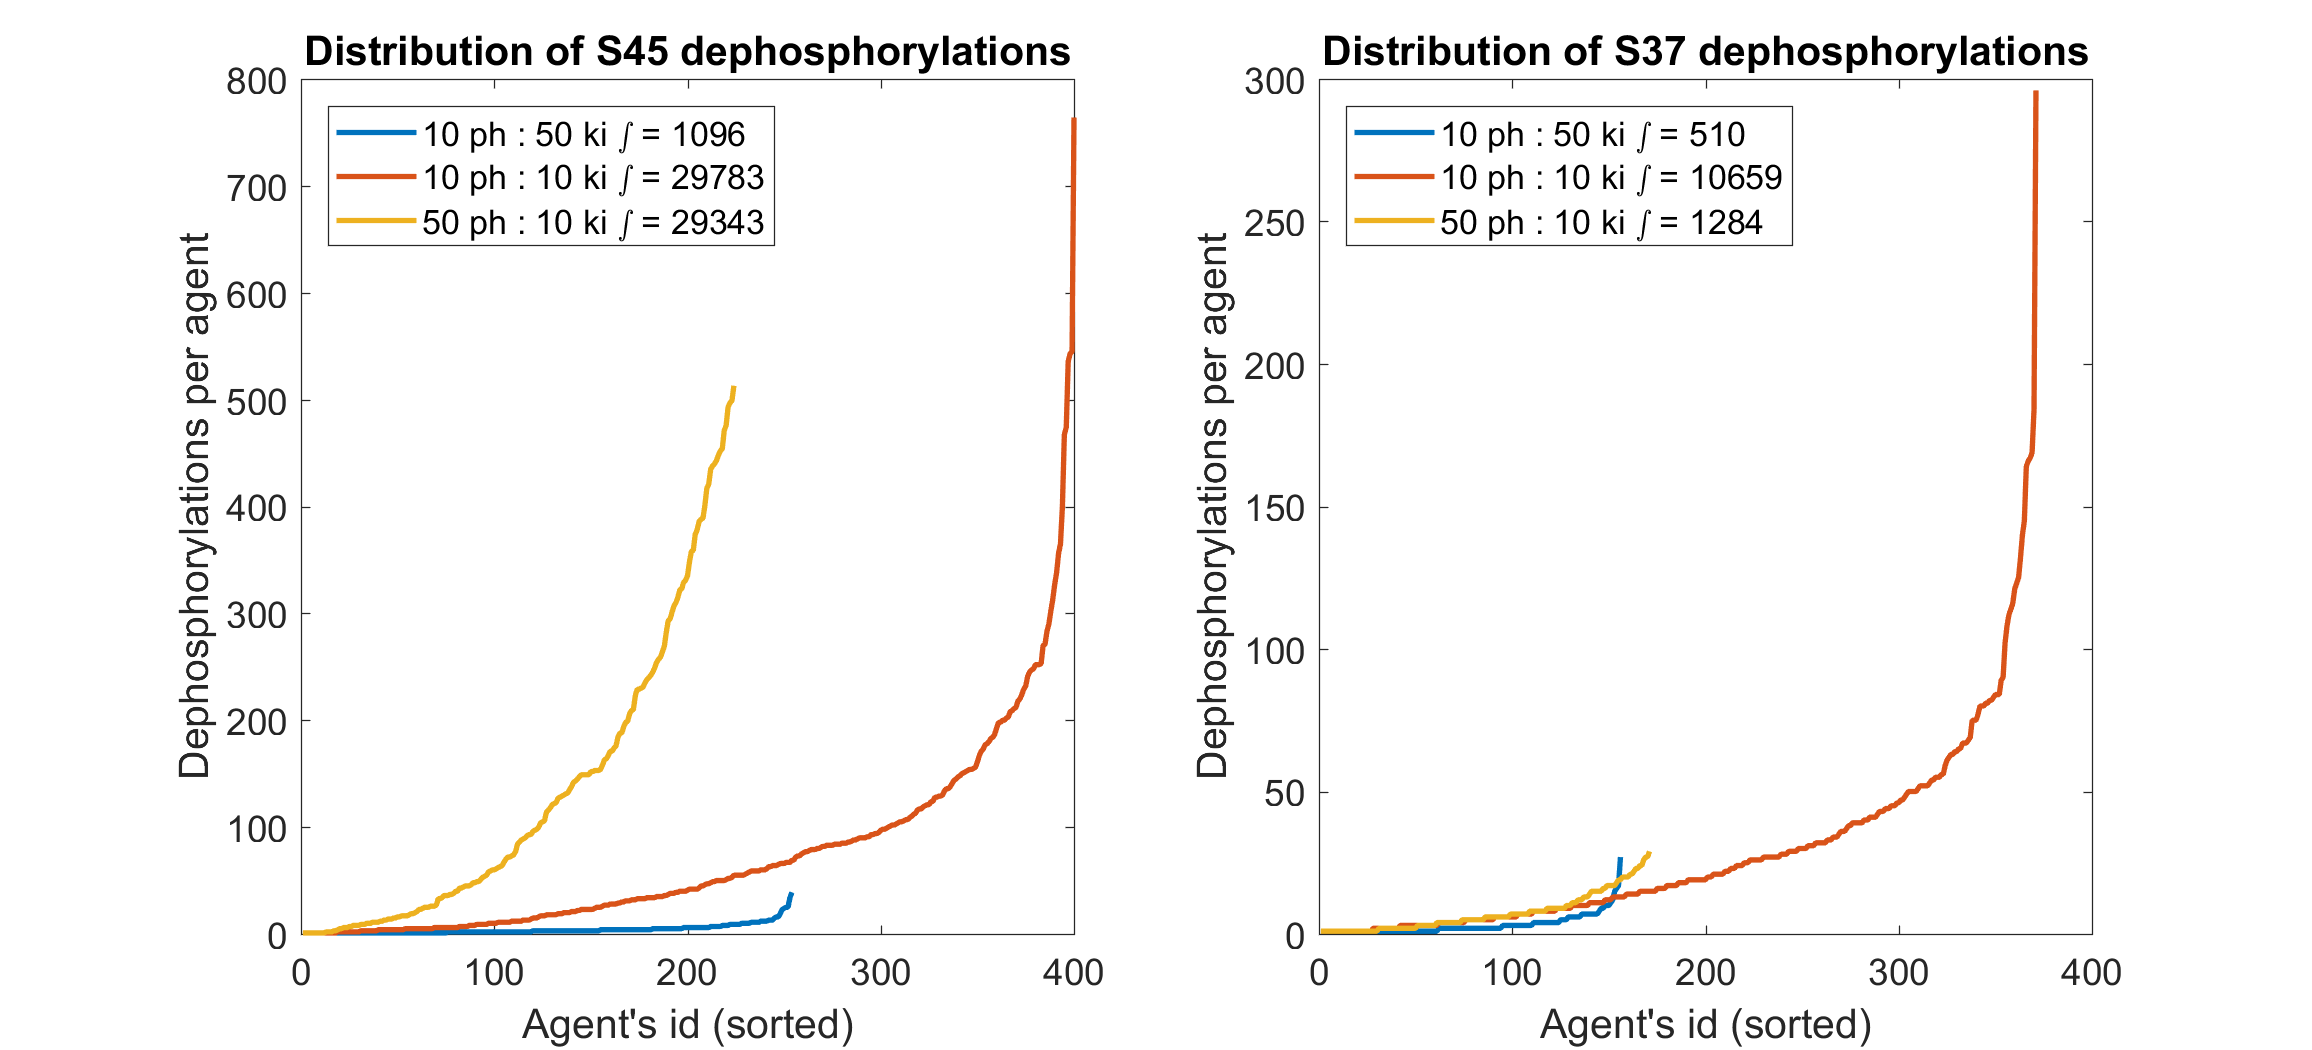
\includegraphics[width=\columnwidth]{wnt/F1_distribution_dephosphorylations_per_agent_brief.png}
  \caption{Distribution of dephosphorylation events per agent. Each
    time an agent gets dephosphorylated, its ID is registered. After
    sorting, we plot the distribution of these IDs for two residues in
    the three parameter regimes. The area under the curve is also
    presented on each legend. S45 is the first residue to get
    phosphorylated, S37 (along with S33) is the last.}
  \label{F1}
\end{figure}


\subsubsection*{Wait times}
Looking at the distribution of wait times (Figure~\ref{F2}), from
first phosphorylation to degradation, we note the bulk of degradation
events occur rapidly, in less than $50$ seconds. Worth noting that,
from the 1:1 regime, increasing the amount of kinase five-fold
marginally reduced wait times.

\begin{figure}[h]
  \centering
  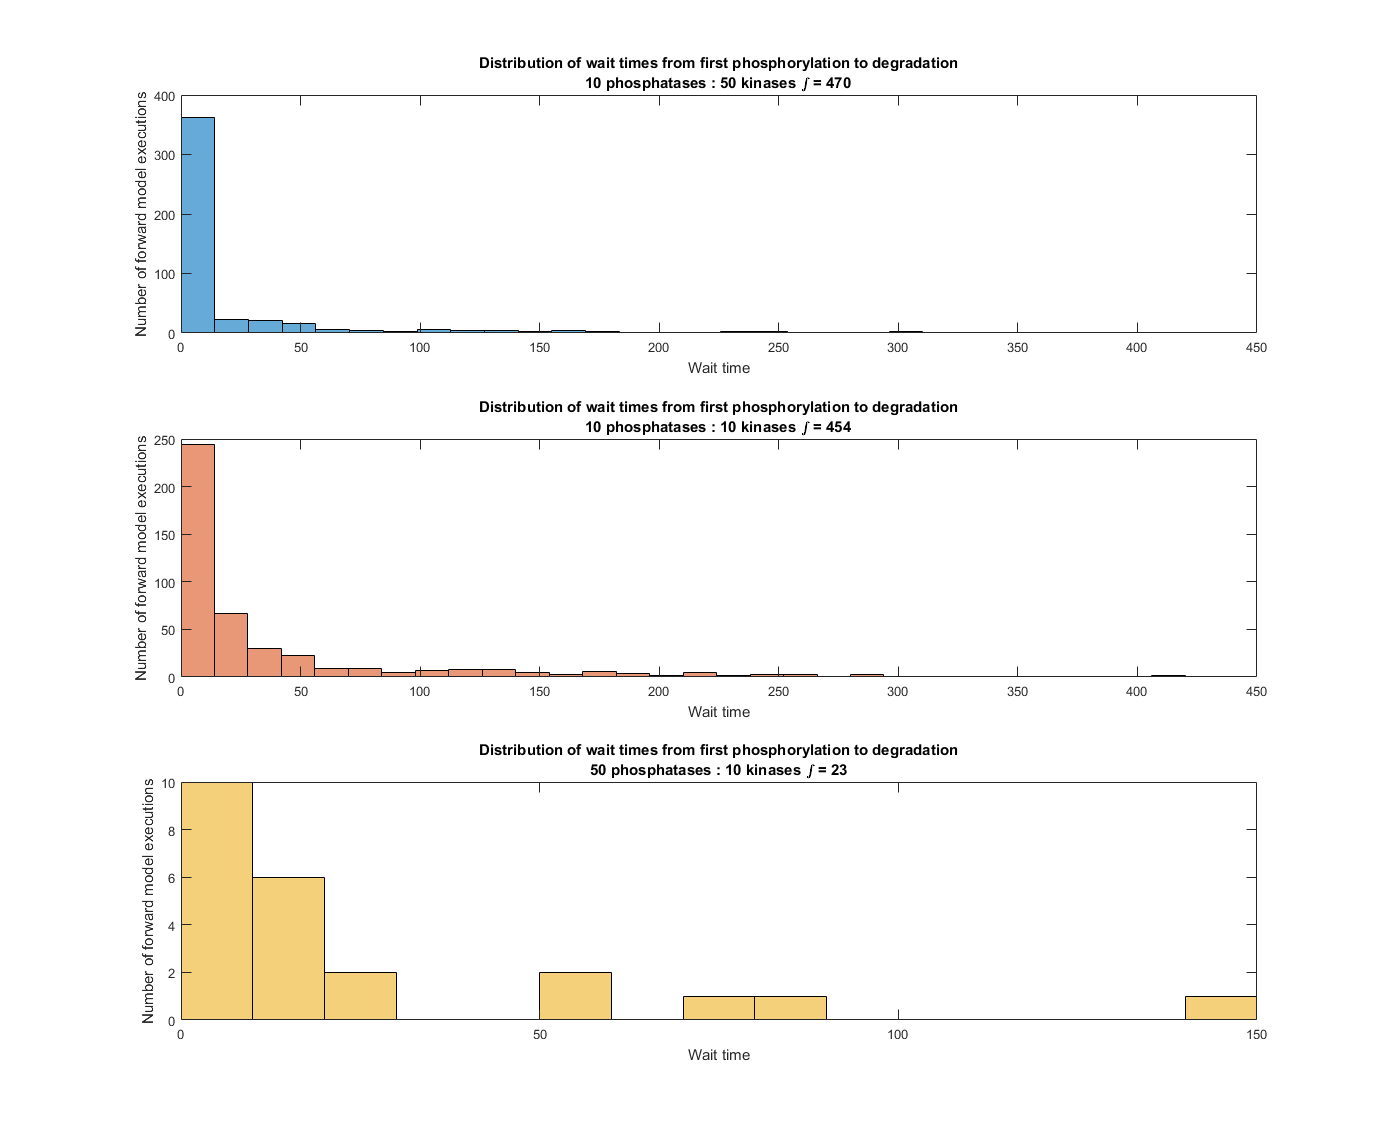
\includegraphics[width=\columnwidth]{wnt/F2_wait_times.png}
  \caption{Distribution of wait times from first phosphorylation until
    degradation. The sum of the bins is presented in the legend of
    each plot, and corresponds to the total number of degradation
    events, matching what is seen on Figure~\ref{F0}. The height of
    each bin represents the number of agents that waited the bin's
    position (in seconds) since they were first modified until they
    were degraded.}
  \label{F2}
\end{figure}


\subsubsection*{Complex composition}

A way of looking at the question of complex contribution is to query
the size of the complex at the last phosphorylation event before
degradation. Taking S45 as representative of all the other residues
(see Figure~\ref{F11} in Appendix~\ref{ap:use-case} for a residue comparative),
we plot the size of the complex, in terms of Axn and APC, at the time
the final S45 occurred. Overall, we see a broad distribution of sizes,
with some phosphorylation events occurring in large complexes
(i.e. $>80$ Axn, $>40$ APC), but a significant number occurring in far
smaller complexes (i.e. $<10$ Axn, $<10$ APC). Changing the parameter
regime of kinase to phosphatase does not seem to alter this behavior
significantly.

\begin{figure}[h]
  \centering
  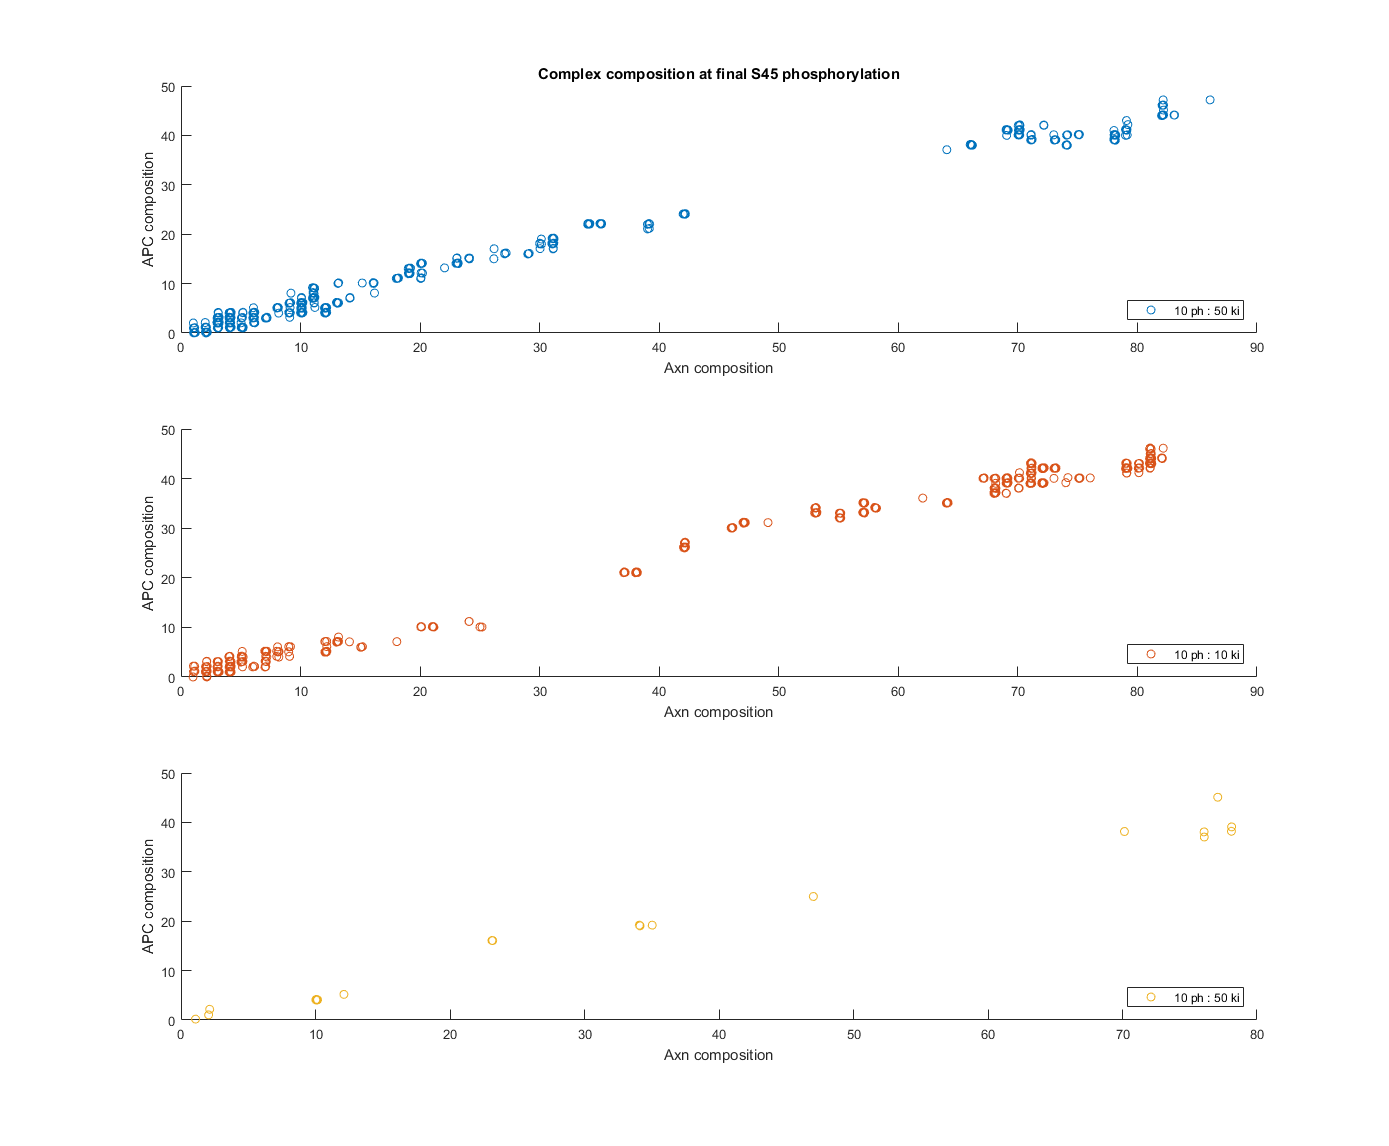
\includegraphics[width=\columnwidth]{wnt/F6_complex_composition_final_S45.png}
  \caption{Composition of the complex, in terms of Axn and APC
    components, at the last event where Cat got S45 phosphorylated
    before being degraded. The number of points corresponds to the number of
    degradation events. The points of this scatter plot have
    been nudged with a random noise factor of 0.2 to increase visual
    perception of discrete points where the data overlap.}
  \label{F6}
\end{figure}


\subsection{Summary of Findings}

\begin{enumerate}
\item The number of undo events does not inform us of overall
  throughput (contrast Figure~\ref{F1} and Figure~\ref{F0}).
\item How a step may be affected by changing abundances depends
  greatly on its upstream context (Figure~\ref{F1}).
\item Entities that got degraded waited a short while since their
  first modification (Figure~\ref{F2}), and yet most modifications
  were futile (Figure~\ref{F1}).
\item We can't argue that giant complexes, nor small complexes, nor
  medium complexes, are the sole entities responsible for performing
  the effective (i.e. final) phosphorylation events  (Figure~\ref{F6}); %F6-9
  the distribution of complexes is wide, and they all contribute to
  the kinetics.
\end{enumerate}

The capacity of querying a simulation's trace offers a mechanistic description of the inner workings of our system. Since this description uses the vocabulary of molecular biology, it can greatly inform the search for drug targets. 

For example, in our setup, complexes with over 60 copies of Axn and over 40 copies of APC contributed a large amount of degradation events (Figure~\ref{F6}). Considering there were a total of 100 copies of each scaffold, these large complexes are giant components, having recruited the majority of scaffolds into a single entity. If a single entity is contributing an amount of degradation events comparable to the rest of the mixture, it means its \emph{effective} catalytic rate is greater than that of smaller entities. One could therefore reduce overall degradation of Cat by destabilizing any of the three scaffold interactions (i.e. Axn-Axn, APC-APC, Axn-APC), without affecting the enzymes directly. Since these enzymes are also involved in metabolism, it would be desirable to avoid affecting their behaviors outside our pathway of interest.